\documentclass{sig-alternate}
\usepackage{amsfonts,xspace}
\usepackage{url}
\usepackage{epsfig}
\usepackage{graphicx}
\usepackage{subfigure}
\usepackage{ifpdf}
\usepackage[usenames,dvipsnames]{color}
\newcommand{\tbd}[1]{}
\newcommand{\ie}{{\it i.e.}}
\newcommand{\eg}{{\it e.g.}}
\newcommand{\etc}{{\it etc.}}
\newcommand{\eat}[1]{}
\usepackage[english,plain]{fancyref}
\usepackage{times}
\usepackage{rotating}
\usepackage[labelformat=simple]{subfig}


\newcommand{\mypara}[1]{\medskip\noindent{\bf {#1}:}~}
\newcommand{\chk}{$\checkmark$}
\newcommand{\dsh}{{\bf --}}
\newcommand{\til}{{\bf\large \textasciitilde}}
%\newcommand{\tbd}[1]{[{\color{red}{\bf{TBD: #1}}}]}
\newcommand{\etal}{\emph{et~al.}}
\newcommand{\meddle}{{\em Meddle}\xspace}
\newcommand{\dsum}{\displaystyle\sum}
\newcounter{packednmbr}

\newenvironment{packedenumerate}{\begin{list}{\thepackednmbr.}{\usecounter{packednmbr}\setlength{\itemsep}{0.2pt}\addtolength{\labelwidth}{-4pt}\setlength{\leftmargin}{\labelwidth}\setlength{\listparindent}{\parindent}\setlength{\parsep}{1pt}\setlength{\topsep}{0pt}}}{\end{list}}
\newenvironment{packeditemize}{\begin{list}{$\bullet$}{\setlength{\itemsep}{0.2pt}\addtolength{\labelwidth}{-4pt}\setlength{\leftmargin}{\labelwidth}\setlength{\listparindent}{\parindent}\setlength{\parsep}{1pt}\setlength{\topsep}{0pt}}}{\end{list}}
\newenvironment{packedtrivlist}{\begin{list}{\setlength{\itemsep}{0.2pt}\addtolength{\labelwidth}{-4pt}\setlength{\leftmargin}{\labelwidth}\setlength{\listparindent}{\parindent}\setlength{\parsep}{1pt}\setlength{\topsep}{0pt}}}{\end{list}}

\renewcommand{\fref}{\Fref}
\renewcommand\thesubfigure{~(\alph{subfigure})}

\title{Meddle: Middleboxes for Increased Transparency and Control of
  Mobile Traffic\vspace{-0.2in}}

% middlebox transparency control mobile traffic 
\numberofauthors{6}
\author{
\alignauthor
Ashwin Rao\\
\affaddr{INRIA}
\alignauthor        
Justine Sherry\\
\affaddr{UC Berkeley}
\alignauthor
Arnaud Legaut\\
\affaddr{INRIA}
\and
\alignauthor 
Arvind Krishnamurthy\\
\affaddr{University of Washington}
\alignauthor
Walid Dabbous\\
\affaddr{INRIA}
\alignauthor
David Choffnes\\
\affaddr{University of Washington}
}
\begin{document}	
%http://www.sheridanprinting.com/typedept/conextstudent.htm
\conferenceinfo{CoNEXT Student'12,} {December 10, 2012, Nice, France.}
\CopyrightYear{2012}
\crdata{978-1-4503-1779-5/12/12}
\clubpenalty=10000
\widowpenalty = 10000

\maketitle

% \begin{abstract}
% In this poster we present \meddle, a framework aimed at enhancing
% the transparency in mobile networks and providing a platform that lets
% users reclaim control over their mobile traffic. We use our working
% prototype to show that \meddle, which builds upon VPNs and
% middleboxes, is feasible to implement, and is capable of providing
% sufficient incentives to conduct large scale experiments and user
% based measurement studies.
% \end{abstract}

\category{C.2}{Computer Communication Networks}{General} 

\begin{keywords}
Middlebox, Mobile, Transparency, Control.
\end{keywords}

\section{Introduction}

Mobile networks are the most popular, fastest growing and least
understood systems in today's Internet ecosystem. Despite a large
collection of privacy, policy and performance issues in mobile
networks~\cite{enck:taintdroid, hornyack:appfence} users and
researchers are faced with few options to characterize and address
them. In this poster we present \meddle, a framework aimed at
enhancing transparency in mobile networks and providing a platform
that enables users (and researchers) control mobile traffic.

In the mobile environment, users are forced to interact with a single
operating system tied to their device, generally run closed-source
apps that routinely violate user privacy~\cite{hornyack:appfence}, and
subscribe to network providers that can (and do) transparently modify,
block or otherwise interfere with network
traffic~\cite{wang:middleboxes}.  

Researchers face a similar set of challenges for characterizing an
and experimenting with mobile systems. To characterize mobile traffic and
design new protocols and services that are better tailored to the
mobile environment, we would like a framework that allows us to
intercept and potentially modify traffic generated by mobile devices
as they move with users, regardless of the device, OS, wireless
technology, or carrier. However, implementing this functionality is
difficult on mobile devices because it requires warranty-voiding
techniques such as jail breaking to access and manipulate traffic at
the network layer~\cite{enck:taintdroid}. Even when using such an
approach, carriers may manipulate traffic once it leaves the mobile
device~\cite{wang:middleboxes}, thus rendering some research
impractical. Furthermore, researchers generally have no ability to 
deploy solutions and services such as prefetching and security
filters, that should be implemented in the network.

In this poster, we present \meddle, a framework that combines Virtual
Private Networks (VPNs) with middleboxes to provide an experimental
platform that aligns the interests of users and researchers. \meddle
relies on VPN tunnels to access the mobile traffic regardless of the
device, OS, wireless technology, and carrier. \meddle can thus provide
a continuous and comprehensive view of how mobile devices interact
with the Internet. Once packets arrive at a \meddle server, we use a
variety of middlebox approaches to interpose on mobile-device
traffic. 

\meddle offers new opportunities for measuring and characterizing
mobile traffic, and designing new in-network features to improve the
mobile experience. For example, by accessing network traffic
regardless of the wireless technology we can analyze how different
operating systems and apps offload their traffic from 3G or 4G
networks to Wi-Fi. To improve the user experience, we implement packet
filters to block ads; unlike existing packet filters for mobile
devices, the packet filter provided by \meddle does not require
jail-breaking the mobile device. Furthermore, Meddle provides a
vantage point for separating mobile-network performance from
server-side performance, thus improving bottleneck identification for
mobile applications. \meddle also enables researchers to investigate
what-if scenarios for the impact of new middleboxes as if they were
deployed in carrier networks. For example, \meddle can be used to
deploy anonymization systems such as Privad~\cite{guha:privad}.  

\section{Meddle Architecture}

\begin{figure}
  \centering
  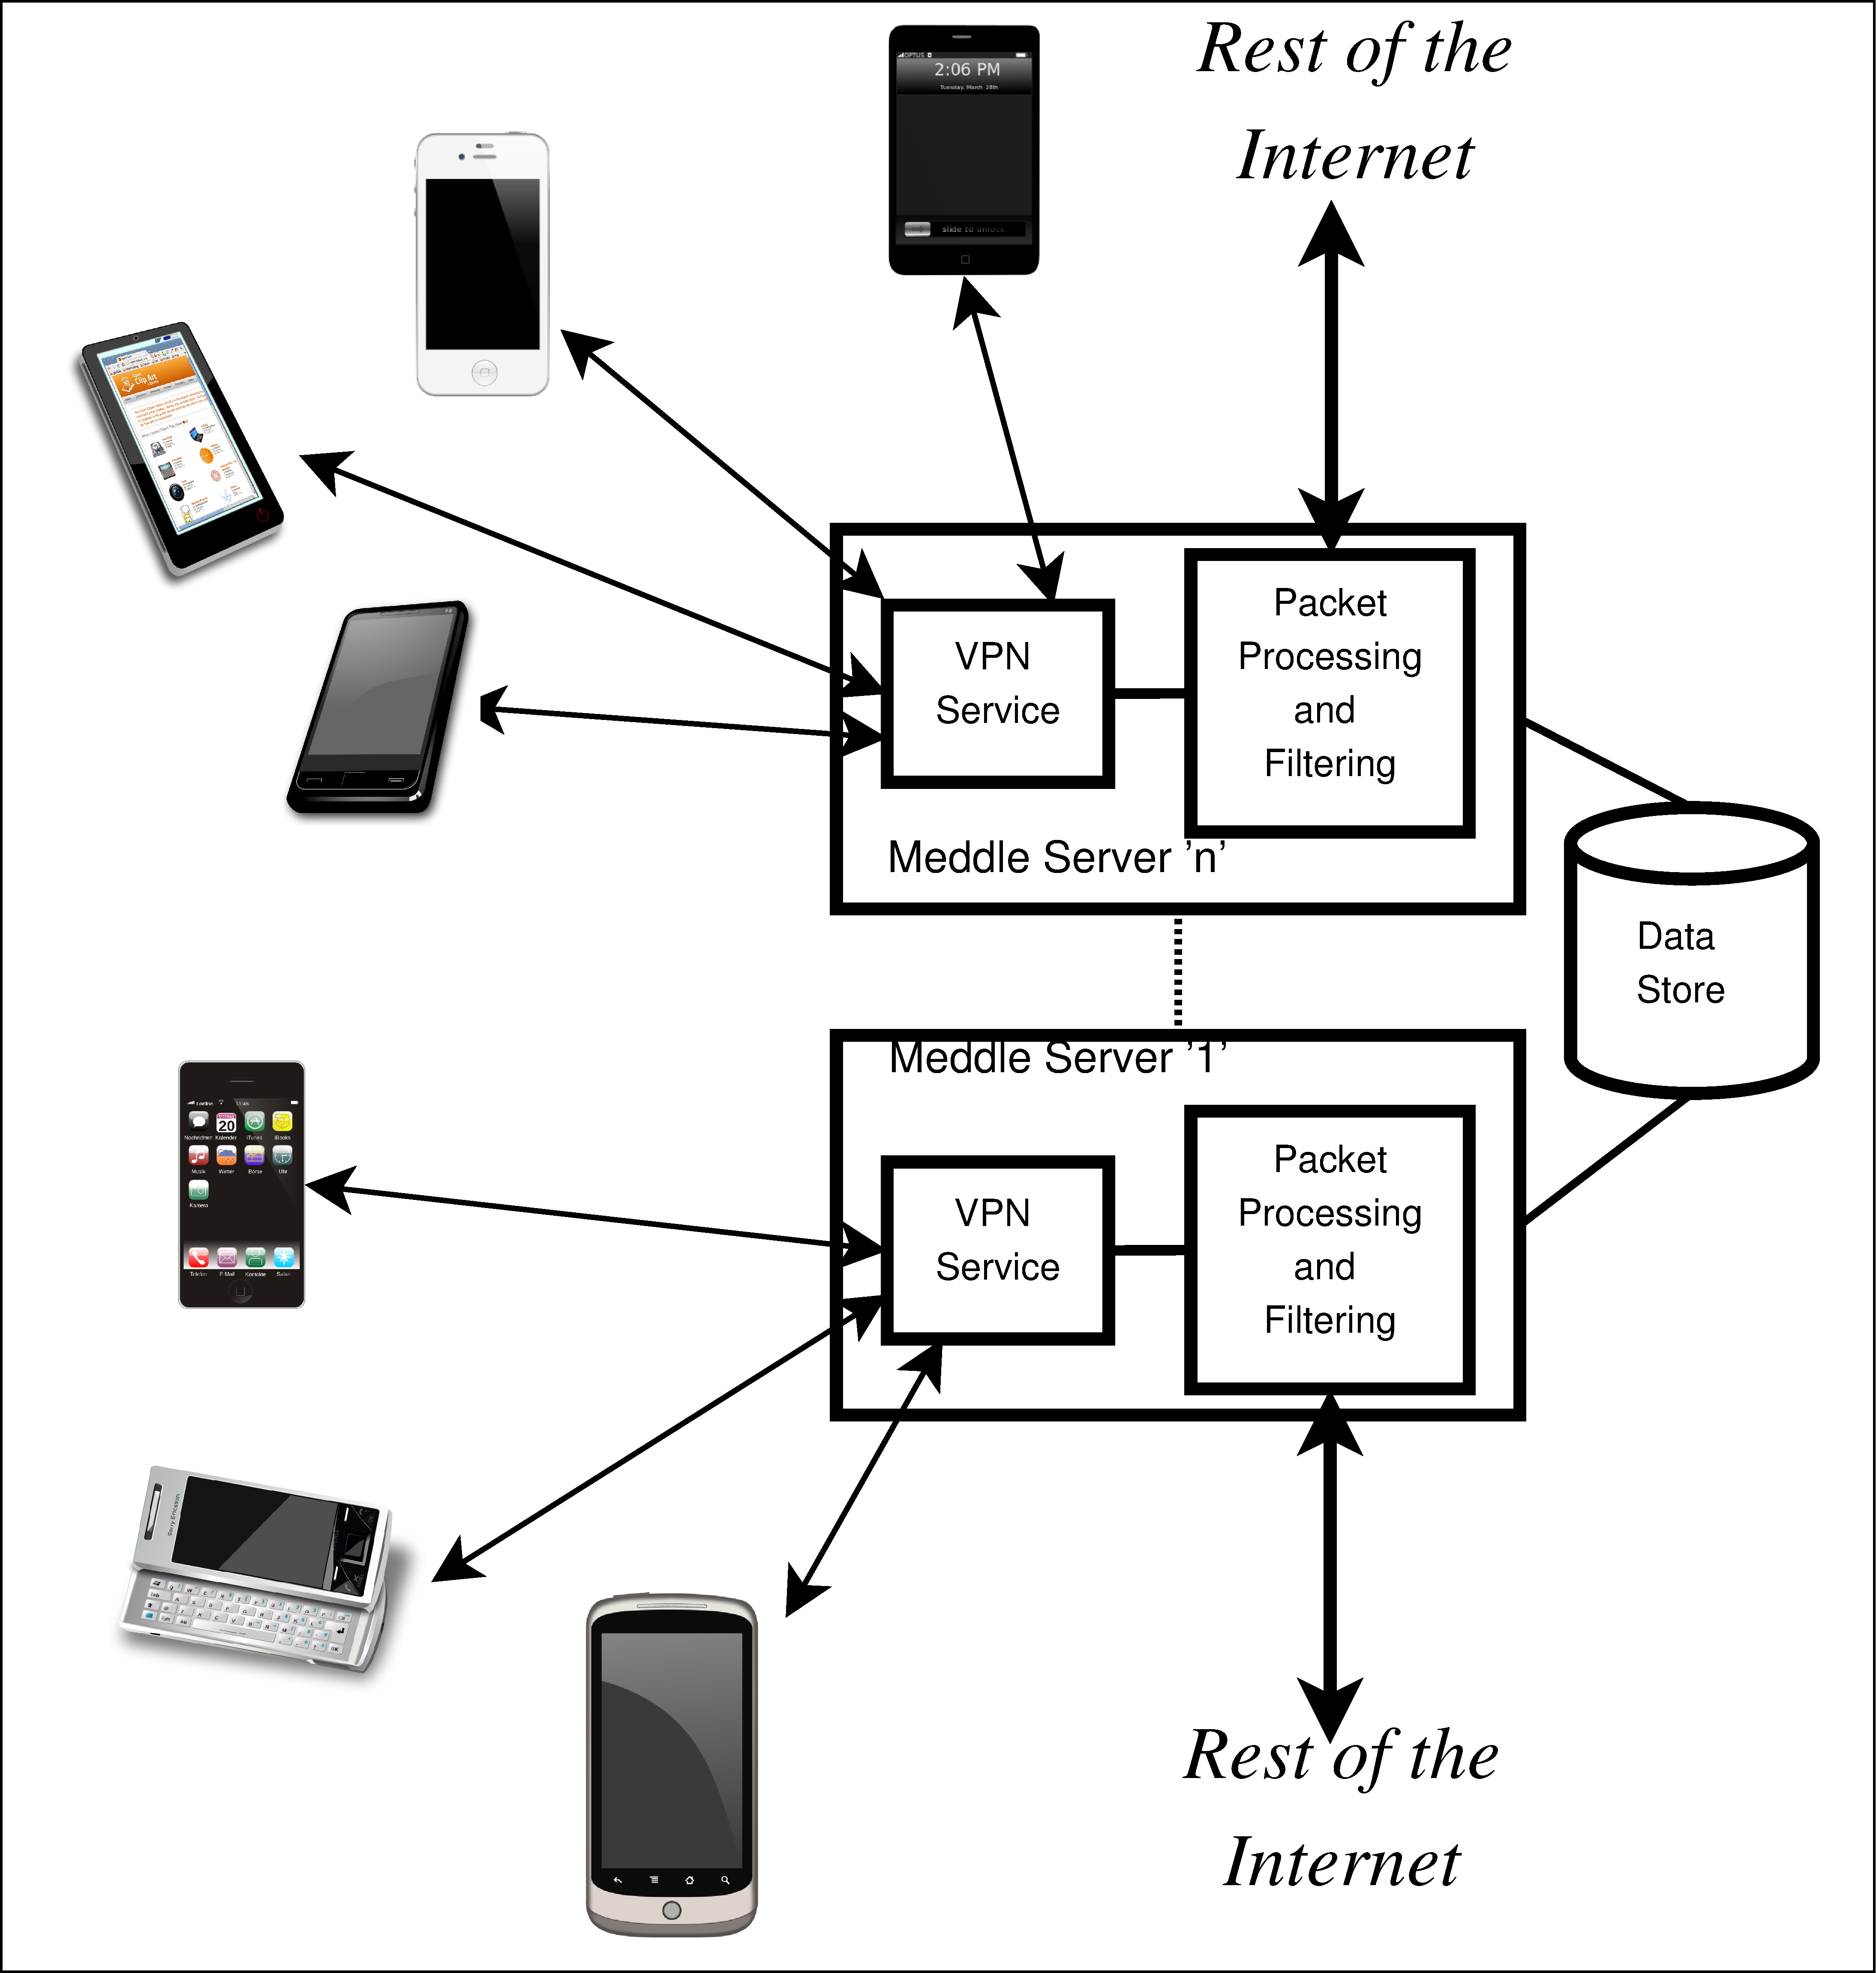
\includegraphics[width=0.75\columnwidth]{figures/meddle-servers.eps}
  \caption{System overview. \emph{Clients use VPNs to connect to a
      nearby \meddle server that interposes traffic.}} 
  \label{fig:MeddleDeployment}
\end{figure}

\meddle uses VPNs as a portable mechanism to tunnel the data traffic
from mobile devices to a machine where users and researchers can exert
control over network flows. VPNs also reduce the barrier to entry for
deploying \meddle because Android, BlackBerry, and iOS, which represent more than 86\% of
the mobile device market~\cite{gartner-phone-share}, have native VPN
support. As shown in \fref{fig:MeddleDeployment}, when a mobile device
connects to the Internet, we tunnel its traffic via a nearby \meddle
server in a similar way to how CDNs use DNS to redirect Web
clients to nearby content caches~\cite{akamai:cdn}. On each
\meddle server we implement custom services for users such as
packet filtering, caching, and intrusion detection. \meddle thus takes
two well-known technologies -- VPNs and middleboxes -- and combines
them in unintended ways for the mobile environment. 
%, and (b) monitor the
%network traffic characteristics

% \meddle requires minimal inputs from end users. For iOS devices, we
% use the iPhone Configuration Utility to generate a user specific
% profile that creates and manages the VPN tunnel. Once the user installs
% this profile, all the data traffic from the iOS  device is tunneled
% through the \meddle servers. For Android devices, we use a modified
% Strongswan app because of some bugs related to reconnection in the
% native VPN  implementation~\cite{OnDemandAndroid}. A user needs to
% enter the credentials for the VPN tunnels only once, during the
% installation of the Strongswan app. To manage VPN tunnels on each
% \meddle server, we use StrongSwan~\cite{strongswan}, an open-source
% VPN implementation that uses native IPsec functionality.   

\section{Case Studies}

We believe that the research enabled by \meddle will form a positive
feedback loop in which new, proven research artifacts become
additional incentives for user adoption, thus enabling further
research. We have a \meddle prototype which has been running
since August 27, 2012. Our prototype currently serves different mobile
devices that include an Android phone, an iPhone, an iPad, and an iPod 
Touch. These devices are being used by users that are part of an
IRB-approved study to characterize mobile traffic.

\textbf{\meddle example.} We have implemented a DNS-based filter to
block ads, analytics, and mediation sites. We believe that such a filter is
an important incentive for a user based study because
Vallina-Rodriguez~\etal~\cite{Vallina-rodriguez:2012:AdCache} observe
that ads account for 5\% of daily traffic from more than 50\% of
Android users in a large European ISP. Our ad blocking engine relies
on the publicly available list of domains for ads and
analytics~\cite{YoyoAds}; we augment this list of domains using the
recent research on mobile ads~\cite{hornyack:appfence,
  Leontiadis:2012:AdsMobile}. We observed a 0.05\% to 0.8\% reduction
in total traffic at each mobile device due to our ad blocking engine.

\begin{table}
\centering
\begin{small}
\begin{tabular}{|l|l|l|l|l|}
\hline
{\bf Device} & {\bf Home} & {\bf Work} & {\bf Mobile} & {\bf Volume}\\
    & {\bf (Wi-Fi)} & {\bf (Wi-Fi)} & {\bf (3G)} & {\bf (MB)}\\
\hline
Android & 38.6\% & 58.7\% & 2.7\%  & 436 MB\\
\hline
iPhone & 47.3\% & 23.1\% & 0.7\%  & 105 MB\\
\hline
iPad & 92.8\% & 7.2\% & N-A  & 812 MB\\
\hline

\end{tabular}
\end{small}
\caption{Traffic share and volume from three devices when using Wi-fi at
  home, Wi-Fi at work, or a 3G connection. \emph{\meddle can be used
    for a plethora of user based studies because it provides a
    comprehensive view of mobile traffic regardless of the access
    technology.}} 
\label{tab:Usage}
\end{table}

\textbf{Measuring Traffic Offload.} In \fref{tab:Usage}, we summarize
the traffic volume observed from an Android phone, an
iPhone, and an iPad, for 15 days since October 16, 2012. The three users
generated 1.35 GB of traffic that passed through our \meddle
server. In \fref{tab:Usage}, we observe that the iPhone user consumes
more 3G bandwidth compared to the Android user. We plan to use this
comprehensive view of network traffic to investigate what fraction of
the 3G traffic can be offloaded to the Wi-fi networks. We also plan to
investigate the usage of apps when multiple access technologies are
simultaneously available. Further, we note that the vast majority of
mobile device traffic is traversing Wi-Fi networks instead of cellular
networks. 

\textbf{Overhead.} We observe low overheads in terms of power
consumption, data quota, and network latency, when tunneling data
traffic via a VPN. We observed a 10\% increase in power consumption
when streaming an HD video from YouTube to an Android device and an
iPhone via one of our \meddle servers. We measured the overhead of the
tunnel in terms of data overhead from IPsec headers and keep-alive
messages, finding that it ranges from 8--12\% for an Android phone and
an iPhone. Our test traffic included Web searches, interaction on
social networks, map searches, playing a game, online shopping,
downloading popular apps, emailing and reading the news. To mitigate
potential additional network delay from routing traffic through
\meddle we envision a DONAR-style deployment where users are
dynamically redirected to a \meddle based on network
conditions and server load~\cite{wendell:donar}. We observe that
PlanetLab nodes have a latency between 3\,ms and 13\,ms, with a median
of 5\,ms from the mobile-network egress points. We used the data
collected from 10 mobile phones located throughout the US for this
measurement study. Thus, when compared to RTTs of 10s or 100s of
milliseconds that exist in mobile networks, the additional latencies
from traversing a \meddle server is expected to be relatively small or
even negligible.  

\section{Future Work}

% \begin{figure}
%  \centering
%  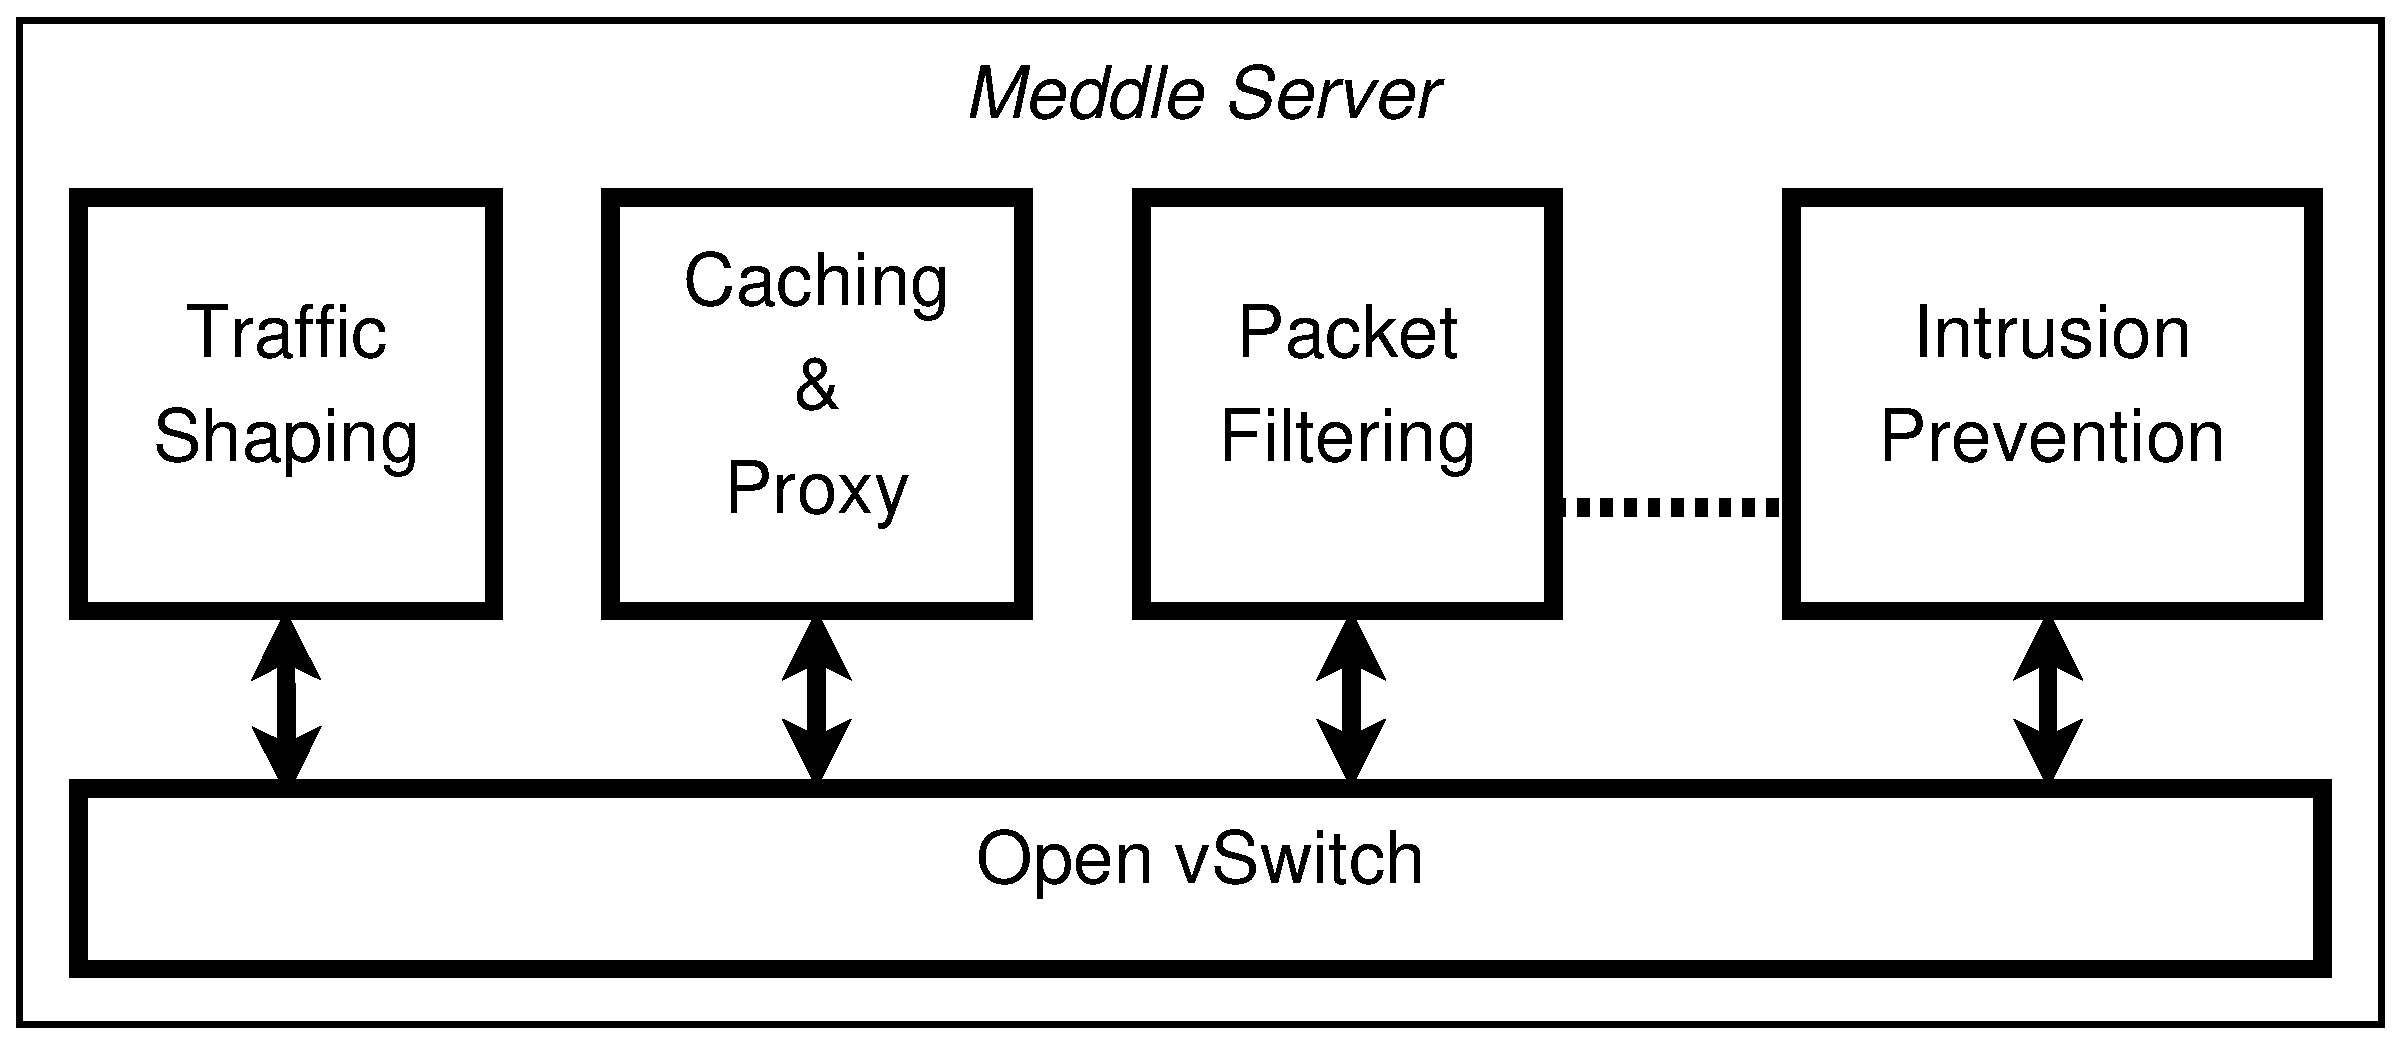
\includegraphics[width=0.65\columnwidth]{figures/OpenSwitch.eps}
%  \caption{Virtual machines on each \meddle server. \emph{Each virtual
%      machine addresses a specific problem.}}
%  \label{fig:OpenSwitch}
% \vspace{-0.09in}
% \end{figure}

We are currently recruiting users for an IRB approved study on the
network usage profiles of mobile phone users. To enhance the
transparency of mobile networks, we plan to allow users to observe how
their installed apps use the network and with whom these apps share (or
leak) information; a system similar to Mozilla
Collusion~\cite{collusion}. 
%We plan on using Open
%vSwitch~\cite{Openvswitch} on each \meddle server to route packets
%through virtual machines depending on the source of the traffic and
%the protocols used to create the
%packets~\cite{Sekar:2012:ConsolidatedMBox}. 
We also plan to test algorithms for content coalescing, caching,
prefetching, and offloading the work of processing the DOM to speed up
page load times~\cite{opera-mini, silk, google-spdy}. We are currently
working towards making the \meddle system publicly available along
with a framework to enable researchers contribute to the \meddle
system and analyze the data collected by the \meddle servers.  

\begin{small}
\bibliographystyle{abbrv}
\bibliography{related_work}
\end{small}
\end{document}
